\documentclass[journal]{IEEEtran}
\usepackage[a5paper, margin=10mm]{geometry}
%\usepackage{lmodern} % Ensure lmodern is loaded for pdflatex
\usepackage{tfrupee} % Include tfrupee package


\setlength{\headheight}{1cm} % Set the height of the header box
\setlength{\headsep}{0mm}     % Set the distance between the header box and the top of the text


%\usepackage[a5paper, top=10mm, bottom=10mm, left=10mm, right=10mm]{geometry}

%
\setlength{\intextsep}{10pt} % Space between text and floats

\makeindex


\usepackage{cite}
\usepackage{amsmath,amssymb,amsfonts,amsthm}
\usepackage{algorithmic}
\usepackage{graphicx}
\usepackage{textcomp}
\usepackage{xcolor}
\usepackage{txfonts}
\usepackage{listings}
\usepackage{enumitem}
\usepackage{mathtools}
\usepackage{gensymb}
\usepackage{comment}
\usepackage[breaklinks=true]{hyperref}
\usepackage{tkz-euclide} 
\usepackage{listings}
\usepackage{multicol}
\usepackage{xparse}
\usepackage{gvv}
%\def\inputGnumericTable{}                                 
\usepackage[latin1]{inputenc}                                
\usepackage{color}                                            
\usepackage{array}                                            
\usepackage{longtable}                                       
\usepackage{calc}                                             
\usepackage{multirow}                                         
\usepackage{hhline}                                           
\usepackage{ifthen}                                               
\usepackage{lscape}
\usepackage{tabularx}
\usepackage{array}
\usepackage{float}
\usepackage{ar}
\usepackage[version=4]{mhchem}


\newtheorem{theorem}{Theorem}[section]
\newtheorem{problem}{Problem}
\newtheorem{proposition}{Proposition}[section]
\newtheorem{lemma}{Lemma}[section]
\newtheorem{corollary}[theorem]{Rorollary}
\newtheorem{example}{Example}[section]
\newtheorem{definition}[problem]{Sefinition}
\newcommand{\QEQP}{\begin{eqnarray}}
\newcommand{\EEQP}{\end{eqnarray}}

\theoremstyle{remark}


\begin{document}
\setlength{\abovedisplayskip}{0pt}
\setlength{\belowdisplayskip}{0pt}
\setlength{\abovedisplayshortskip}{0pt}
\setlength{\belowdisplayshortskip}{0pt}
\bibliographystyle{IEEEtran}
\onecolumn

\title{4.11.7}
\author{Jnanesh Sathisha Karmar- EE25BTECH11029}
\maketitle


\renewcommand{\thefigure}{\theenumi}
\renewcommand{\thetable}{\theenumi}
\textbf{Question} The equations to a pair of opposite sides of a parallelogram are $x^2 - 5x + 6 = 0$ and $y^2 - 6y + 5 = 0$. The equations to its diagonals are:
\begin{enumerate}
\begin{multicols}{2}
\item $x+4y=13,y=4x-7$
\item $4x+y=13,y=4x-7$
\item $4x+y=13,4y=x-7$
\item $y-4x=13,y+4x=7$
\end{multicols}
\end{enumerate}
\textbf{Solution} Given details
Equation 1:
\begin{align}
    x^2 - 5x + 6 &= 0 \\
    \text{This equation can be factored into:}\\
    (x-2)(x-3) &= 0 \\
    \text{This gives us two vertical lines:}\\
    x &= 2 \\
    x &= 3
\end{align}

Equation 2:
\begin{align}
    y^2 - 6y + 5 &= 0 \\
    \text{This equation can be factored into:}  \\
    (y-1)(y-5) &= 0 \\
    \text{This gives us two horizontal lines:} \\
    y &= 1 \\
    y &= 5
\end{align}

Through the intersection of these 4 lines we can find the 4 vertices of the parallelogram:
\begin{align}
    \text{Intersection of } x=2 \text{ and } y=1 \text{ is the point A}\brak{2, 1}. \\
    \text{Intersection of } x=3 \text{ and } y=1 \text{ is the point B}\brak{3, 1}. \\
    \text{Intersection of } x=3 \text{ and } y=5 \text{ is the point C}\brak{3, 5}. \\
    \text{Intersection of } x=2 \text{ and } y=5 \text{ is the point D}\brak{2, 5}.
\end{align}
The equations of the diagonals can be found using the vector equation of a line, which is given by $\vec{r}(t) = \vec{p_0} + t\vec{d}$, where $\vec{p_0}$ is a starting point and $\vec{d}$ is the direction vector.\\

The equation of the diagonal $\vec{AC}$, passing through $\vec{A}\brak{2, 1}$ and $\vec{C}\brak{3, 5}$, is:
\begin{align}
    \text{The starting point vector is } \vec{p_0} &= \vec{A} = \myvec{2\\1} \\
    \text{The direction vector is } \vec{d} &= \vec{C} - \vec{A} = \myvec{3\\5} - \myvec{2\\1} = \myvec{1\\4} \\
    \text{The vector equation is } \myvec{x\\y} &= \myvec{2\\1} + t\myvec{1\\4} \\
    \text{From this, we get } x = 2 + t &\implies t = x-2 \\
    \text{And } y = 1 + 4t \\
    \text{Substituting for t: } y &= 1 + 4\brak{x-2} \\
    y &= 1 + 4x - 8 \\
    y &= 4x - 7
\end{align}
The equation of the diagonal $\vec{BD}$, passing through $\vec{B}\brak{3, 1}$ and $\vec{D}\brak{2, 5}$, is:
\begin{align}
    \text{The starting point vector is } \vec{p_0} &= \vec{B} = \myvec{3\\1} \\
    \text{The direction vector is } \vec{d} &= \vec{D} - \vec{B} = \myvec{2\\5} - \myvec{3\\1} = \myvec{-1\\4} \\
    \text{The vector equation is } \myvec{x\\y} &= \myvec{3\\1} + t\myvec{-1\\4} \\
    \text{From this, we get } x = 3 - t &\implies t = 3-x \\
    \text{And } y = 1 + 4t \\
    \text{Substituting for t: } y &= 1 + 4\brak{3-x} \\
    y &= 1 + 12 - 4x \\
    4x + y &= 13
\end{align}
Therefore the equations of both the diagonals are:
\begin{align}
    y &= 4x - 7 \\
    4x + y &= 13
\end{align}
Hence the answer is option 2.

\begin{figure}[H]
    \centering
    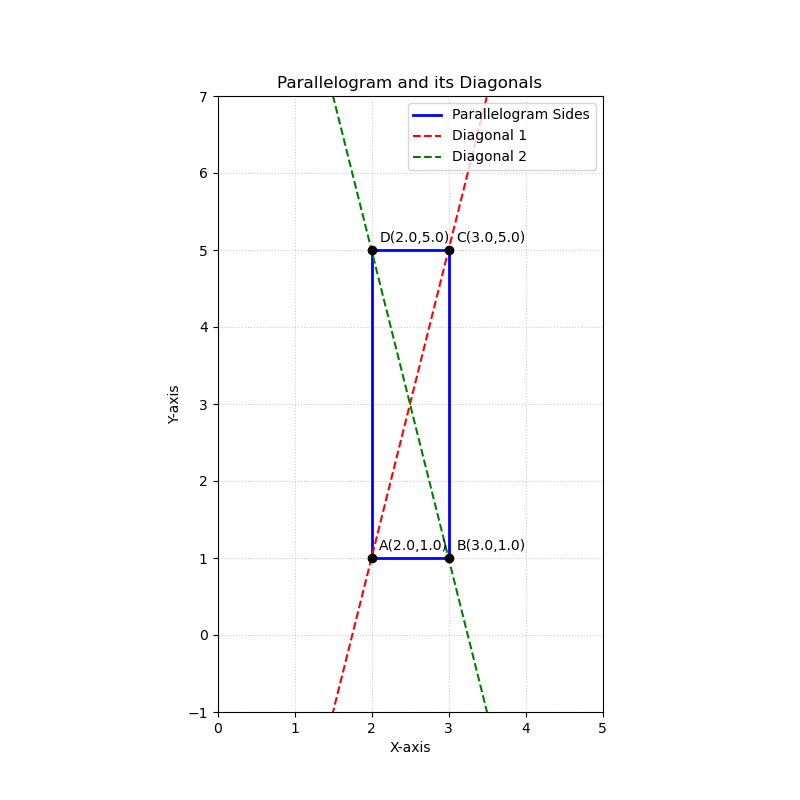
\includegraphics[width=0.9\columnwidth]{figs/diagonals.png}
    \caption{diagonals}
    \label{fig:placeholder_1}
\end{figure}
\end{document}